\documentclass[mathserif,notheorems, hyperref={colorlinks, citecolor=blue, urlcolor=blue, linkcolor=blue}]{beamer}

\usepackage{amsmath}
\usepackage{amssymb}
\usepackage[scale=2]{ccicons}
\usepackage{appendixnumberbeamer}
\usepackage{booktabs}
\usepackage[toc,page]{appendix}
\usepackage{graphicx}
\usepackage{xspace}
\usepackage{adjustbox, lipsum}
\usepackage{bbm}
\usepackage{algorithm}
\usepackage{algpseudocode}
\usepackage[sort]{natbib}

% absolute positioning
\usepackage[absolute,overlay]{textpos}

%% source for images.
\newcommand{\source}[1]{{\let\thefootnote\relax\footnote{{\tiny #1}}}}

\pdfstringdefDisableCommands{%
  \def\\{}%
  \def\texttt#1{<#1>}%
}

\makeatletter
\let\save@measuring@true\measuring@true
\def\measuring@true{%
  \save@measuring@true
  \def\beamer@sortzero##1{\beamer@ifnextcharospec{\beamer@sortzeroread{##1}}{}}%
  \def\beamer@sortzeroread##1<##2>{}%
  \def\beamer@finalnospec{}%
}
\makeatother

\input{macros/math}
%% Originally written by Frederik Kunstner <kunstner@cs.ubc.ca>
%% Modified by Aaron Mishkin <amishkin@cs.ubc.ca>

\usepackage{mdframed}
\mdfdefinestyle{mdframedprocedure}{%
    linewidth=0.05em,
    frametitlerulewidth=0.05em,
	leftmargin=.1\textwidth,
	rightmargin=.1\textwidth,
    frametitlefont=\Large\bfseries,
	frametitlerule=true,
	frametitlealignment=\centering,
	frametitleaboveskip=3ex,
	frametitlebelowskip=3ex,
	innertopmargin=\baselineskip,
    innerbottommargin=\baselineskip,
	innerleftmargin=.5em,
	innerrightmargin=1.5em,
}

\newenvironment{procedure}[1]
	{%
        \large%
        \begin{mdframed}[style=mdframedprocedure, frametitle={#1}]%
		\begin{enumerate}
		\setcounter{enumi}{-1} 
	}{% 
		\end{enumerate}%
		\end{mdframed}%
	}

\usepackage{simplebeam}

%% tikz

\usepackage{tikz}
\usepackage{pgfplots}
\usepgfplotslibrary{fillbetween}
\usetikzlibrary{patterns}
%% pgf and tikz options.
\pgfplotsset{
    compat=1.5.1,
    oracle/.style={color=red, style=dashed, line width=1.5pt},
    bound/.style={color=blue, style=solid, line width=1.5pt},
    objective/.style={color=black, style=solid, line width=1.5pt},
}

\tikzset{
    font={\fontsize{18pt}{12}\selectfont},
}


\title{}
\author{}
\institute{}
\date{}


\begin{document}
    %% TODO: Should write custom title template instead of this slide.
    \setbeamercolor{background canvas}{bg=lightcyan}
        \begin{frame}
        \vspace{1em}
        \begin{center}
            {\Large Interpolation, Growth Conditions, and Stochastic Gradient Descent  \vspace{1em}} %% title

            {\large Aaron Mishkin, \\ \texttt{amishkin@cs.ubc.ca} } %% author
        \end{center}

        \vspace{1ex}

       \begin{figure}
            \centering
            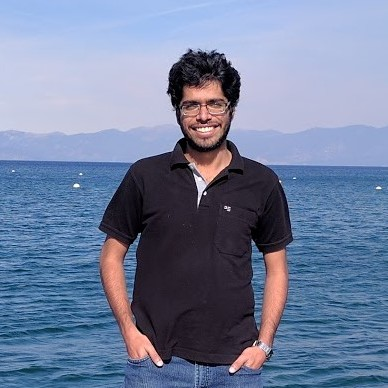
\includegraphics[width=0.18\textwidth]{collaborators/sharan}
            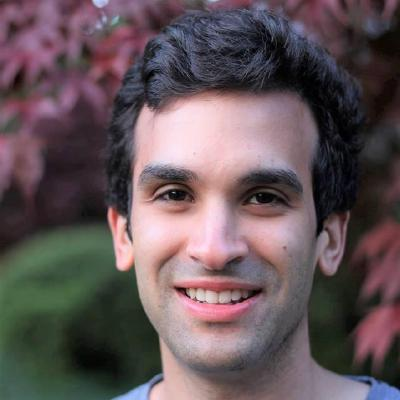
\includegraphics[width=0.18\textwidth]{collaborators/issam}
            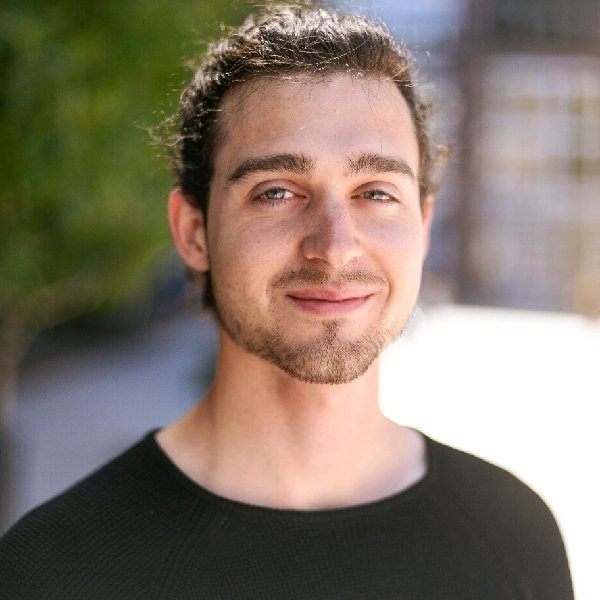
\includegraphics[width=0.18\textwidth]{collaborators/gauthier}
            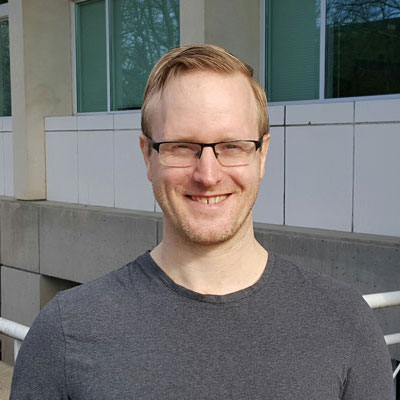
\includegraphics[width=0.18\textwidth]{collaborators/mark}
            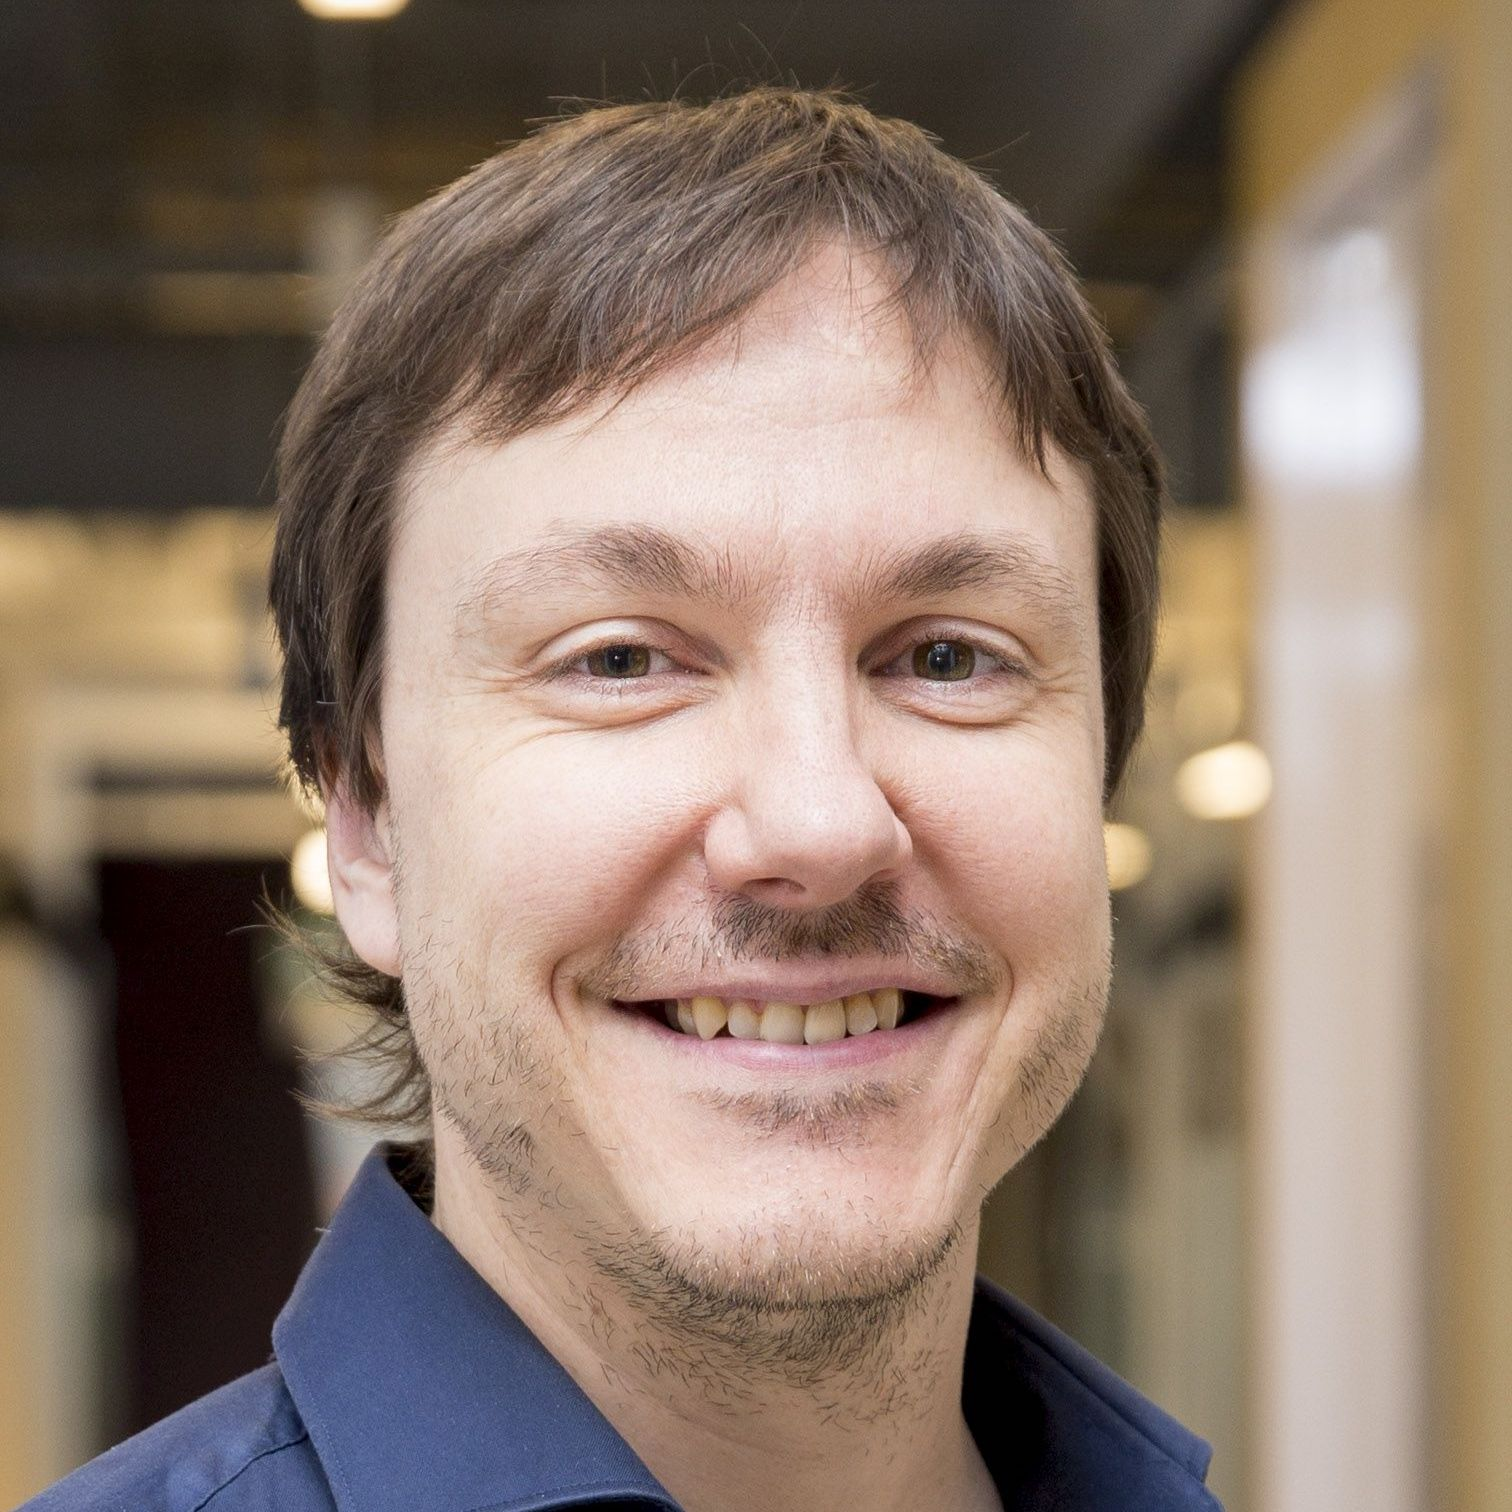
\includegraphics[width=0.18\textwidth]{collaborators/simon}

            \vspace{0.4ex}%

            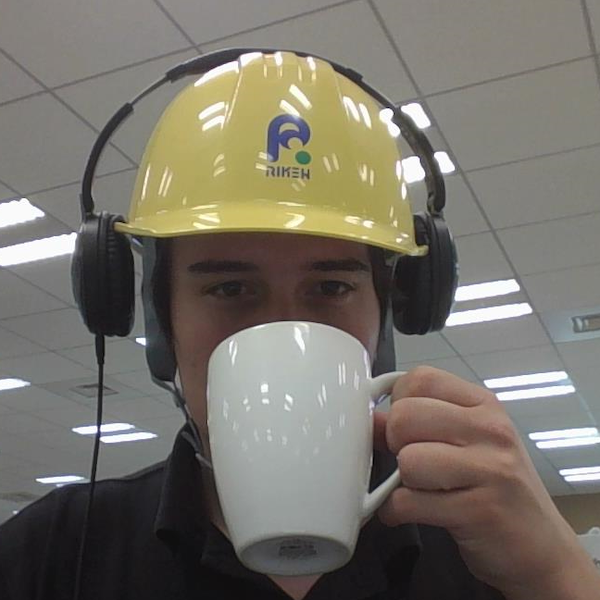
\includegraphics[width=0.18\textwidth]{collaborators/fred}
            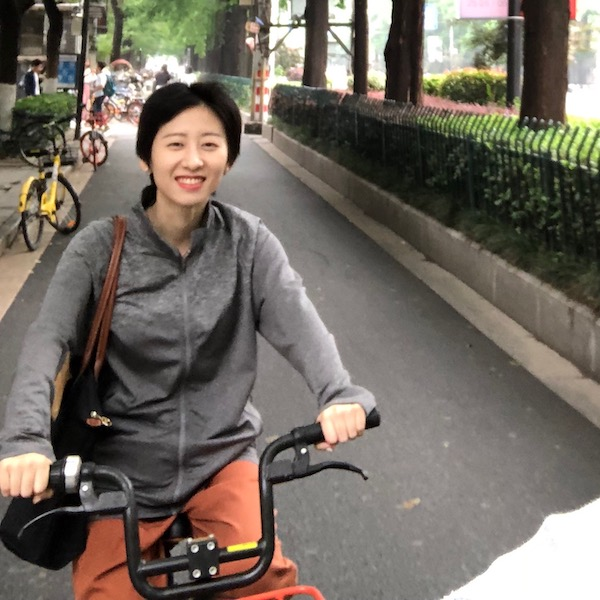
\includegraphics[width=0.18\textwidth]{collaborators/cathy}
            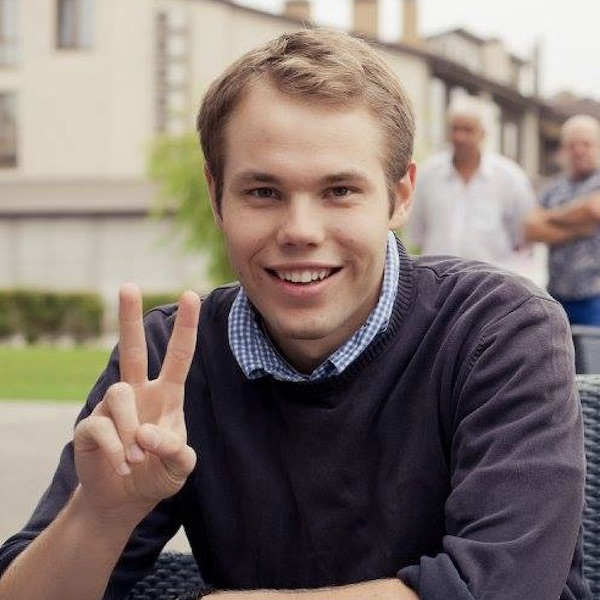
\includegraphics[width=0.18\textwidth]{collaborators/wilder}
            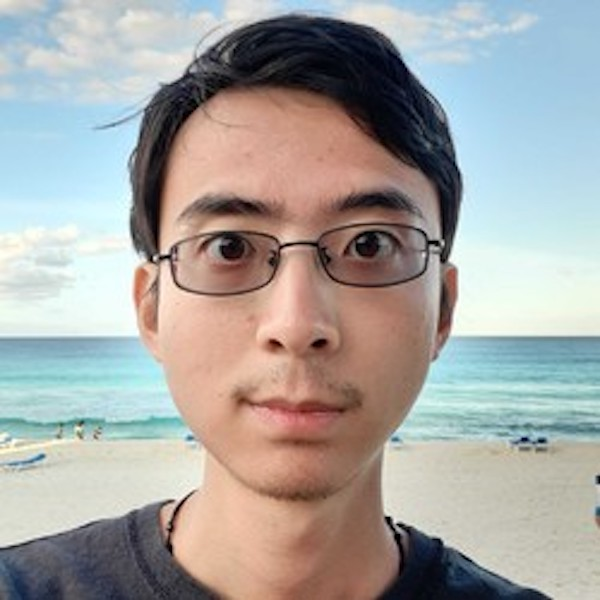
\includegraphics[width=0.18\textwidth]{collaborators/joey}
        \end{figure}
    \end{frame}
   
    \setbeamercolor{background canvas}{bg=white}
  
    \begin{frame}{Training neural networks is dangerous work!}
       
       \begin{figure}
            \centering
            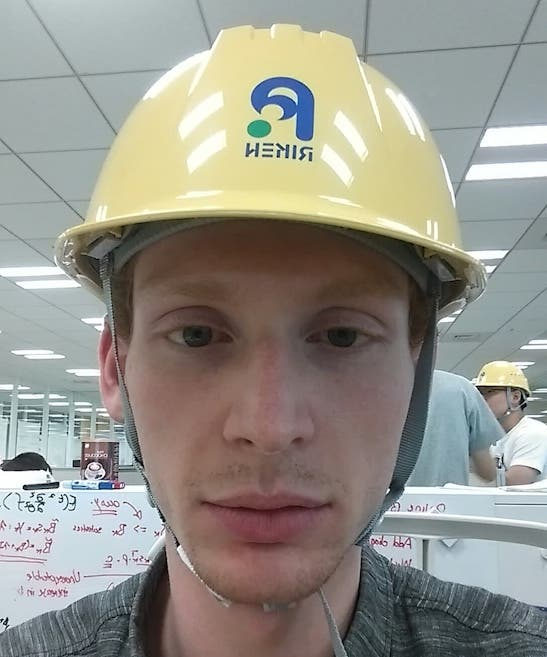
\includegraphics[width=0.45\textwidth]{collaborators/helmet1} 
            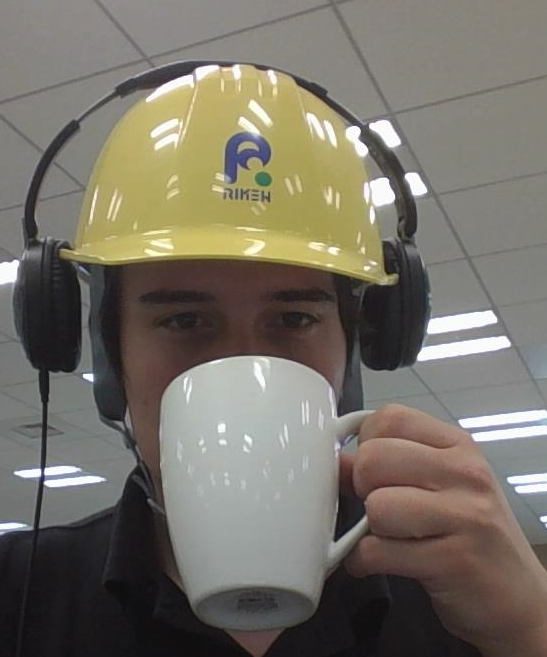
\includegraphics[width=0.45\textwidth]{collaborators/helmet2} 
       \end{figure} 
    \end{frame}
  
    \setbeamercolor{background canvas}{bg=lightcyan}

    \begin{frame}
       \begin{center}
           \Huge Chapter 1: Introduction
       \end{center} 
    \end{frame}

    \setbeamercolor{background canvas}{bg=white}

    \begin{frame}{Chapter 1: Goal}
        \Large 
        
        \textbf{Premise}: modern neural networks are extremely flexible and can exactly fit many training datasets. 
        \begin{itemize}
            \item e.g. ResNet-34 on CIFAR-10. 
        \end{itemize}        

        \vspace{4ex} 

        \textbf{Question}: what is the complexity of learning these models using stochastic gradient descent (SGD)?% 
        
    \end{frame}

    \begin{frame}{Chapter 1: Model Fitting in ML}
       
       \begin{figure}
            \centering
            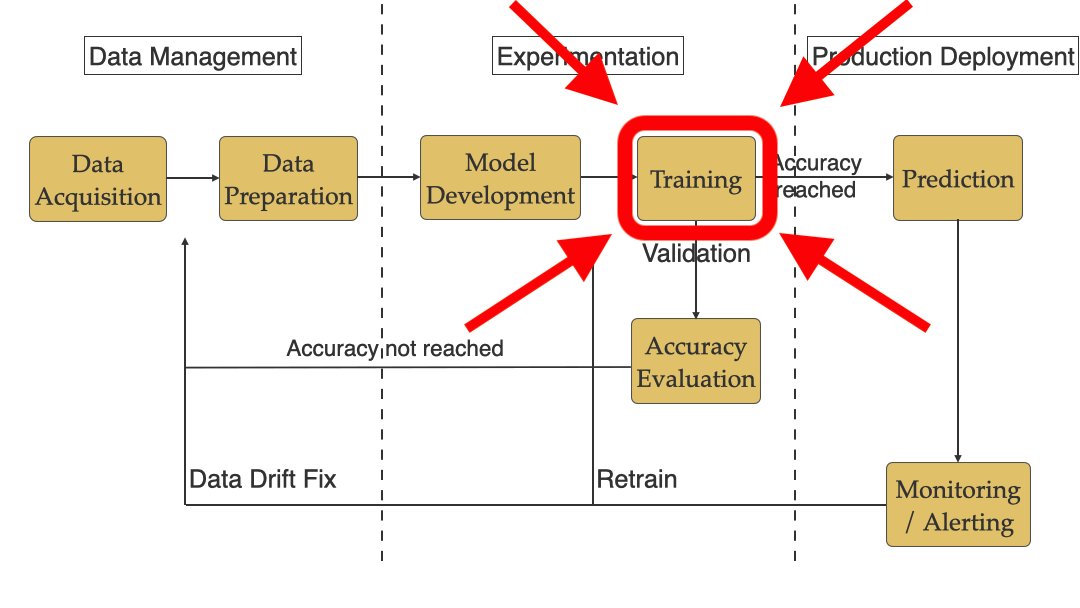
\includegraphics[width=0.98\textwidth]{figures/workflow_highlighted} 
       \end{figure} 

       \source{https://towardsdatascience.com/challenges-deploying-machine-learning-models-to-production-ded3f9009cb3}
    \end{frame}
    
    \begin{frame}{Chapter 1: Stochastic Gradient Descent}

        \begin{center}
            \Large
            ``Stochastic gradient descent (SGD) is today one of the main workhorses for solving large-scale supervised learning and optimization problems.''\\
            ---\citet{drori2019complexity}
        \end{center}

    \end{frame}

    \begin{frame}{Chapter 1: Consensus Says\ldots}

        \begin{center}
            \Large \dots and also~\citet{xu2017second,
            zhang2016parallel,
            patterson2017deep,
            pillaud2018statistical,
            grosse2015scaling,
            assran2018stochastic,
            damaskinos2019aggregathor,
            kawaguchi2020ordered,
            bernstein2018signsgd,
            li2019rsa,
            agarwal2017second,
            hofmann2015variance,
            geffner2019rule,
            assran2020convergence,
            gower2019sgd}
        \end{center}

    \end{frame}

    \begin{frame}{Chapter 1: Challenges in Optimization for ML}

        \textbf{Stochastic gradient methods} are the most popular algorithms for fitting ML models,
        \begin{align*}
            \textbf{SGD:} \quad w_{k + 1} = w_k - \eta_k \nabla f_i \, (w_k). \\
        \end{align*}

        % SGD is scalable and converges if $\eta_k$ decreases sufficiently slowly.\vspace{1em}

        But practitioners face major challenges with \vspace{0.5em}
        \begin{itemize}
            \item \textbf{Speed}: step-size/averaging controls convergence rate.
            \item \textbf{Stability}: hyper-parameters must be tuned carefully.
            \item \textbf{Generalization}: optimizers encode statistical tradeoffs.
        \end{itemize}
        \vspace{1em}

    \end{frame}


    \begin{frame}{Chapter 1: Challenges in Optimization for ML}

        \textbf{Stochastic gradient methods} are the most popular algorithms for fitting ML models,
        \begin{align*}
            \textbf{SGD:} \quad w_{k + 1} = w_k - \eta_k \nabla f_i \, (w_k). \\
        \end{align*}

        % SGD is scalable and converges if $\eta_k$ decreases sufficiently slowly.\vspace{1em}

        But practitioners face major challenges with \vspace{0.5em}
        \begin{itemize}
            \item \textcolor{red}{\textbf{Speed}: step-size/averaging controls convergence rate.}
            \item \textcolor{red}{\textbf{Stability}: hyper-parameters must be tuned carefully.}
            \item \textbf{Generalization}: optimizers encode statistical tradeoffs.
        \end{itemize}
        \vspace{1em}

    \end{frame}


    \begin{frame}{Chapter 1: Better Optimization via Better Models}

        \begin{figure}
            \centering
            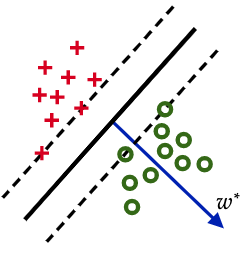
\includegraphics[width=0.38\textwidth]{figures/separable}
            \hspace{0.2em}
            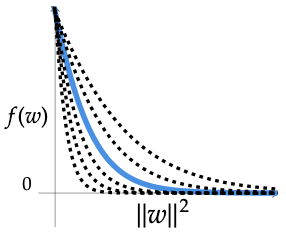
\includegraphics[width=0.45\textwidth]{figures/loss_fn}
        \end{figure}
        \vspace{0.2em}

        \begin{center}
            \large \textbf{Idea}: exploit ``over-parameterization'' for better optimization.
        \end{center}
        \begin{itemize}
            \item Intuitively, gradient noise goes to $0$ if all data are fit exactly.
            \item No need for decreasing step-sizes, or averaging for convergence. 
        \end{itemize}

    \end{frame}

    \setbeamercolor{background canvas}{bg=lightcyan}

    %% interpolation

    \begin{frame}
       \begin{center}
          \huge Chapter 2: Interpolation and Growth Conditions 
       \end{center} 
    \end{frame}

    \setbeamercolor{background canvas}{bg=white}

    \begin{frame}{Chapter 2: Assumptions}
        \begin{center}
            We need assumptions to analyze the complexity of SGD. 
        \end{center}
       
        \vspace{1.5ex}

        \textbf{Goal}: Minimize \( f : \R^d \rightarrow \R \), where
        \vspace{0.5ex}
        \begin{itemize}
            \item \( f \) is \textbf{lower-bounded}: \( \exists \, \wopt \in \R^d \) such that
                \begin{align*}
                    f(\wopt) &\leq f(w) \hspace{1.7em} \tag*{\(\forall \w \in \R^d \), } 
                \end{align*}

            \item \( f \) is L-\textbf{smooth}: \( \w \mapsto \grad(\w) \) is \( L \)-Lipschitz, 
                \begin{align*}
                    \norm{\grad(\w) - \grad(u)}_2 &\leq L \norm{\w - u}_2 \tag*{\(\forall \w, u \in \R^d \),} 
                \end{align*}

            \item (Optional) \( f \) is \( \mu \)-\textbf{strongly-convex}: \( \exists \, \mu \geq 0 \) such that, 
                \begin{align*}
                   f(u) \geq f(\w) + \abr{\grad(\w), u - \w} + \frac{\mu}{2} \norm{u - \w}^2_2 \tag*{\( \forall \w, u \in \R^d \).}
                \end{align*}
        \end{itemize}
     
    \end{frame}

    \begin{frame}{Chapter 2: Stochastic First-Order Oracles}

        \textbf{Stochastic Oracles}:
        \begin{enumerate}
            \item At each iteration \( k \), query oracle \oracle{} for stochastic estimates 
                \[ f(\wk, \zk) \quad \text{and} \quad \grad(\wk, \zk). \] 
            \item \( f(\wk, \cdot) \) is a deterministic function of random variable \( \zk \). 
                \vspace{1ex}
            \item \textcolor{red}{\oracle{} is \textbf{unbiased}}, meaning 
            \[ \Ek\sbr{f(\wk, \zk)} = f(\wk) \quad \text{and} \quad \Ek\sbr{\grad(\wk, \zk)} = \grad(\wk). \]% 
            \item \textcolor{blue}{\oracle{} is \textbf{individually-smooth}}, meaning \( f(\cdot, \zk) \) is \( \Lmax \)-smooth, 
                \begin{align*}
                    \norm{\grad(\w, \zk) - \grad(u, \zk)}_2 &\leq \Lmax \norm{\w - u}_2 \tag*{\(\forall \w, u \in \R^d \),} 
                \end{align*}
                almost surely.
        \end{enumerate}

    \end{frame}

    \begin{frame}{Chapter 2: Defining Interpolation}
        \begin{minipage}{0.72\textwidth}
        \vspace{-5.25ex}
            \begin{restatable}[Interpolation: Minimizers]{definition}{interpolationMinima}\label{def:interpolation-minima}
                \( (f, \oracle{}) \) satisfies minimizer interpolation if 
                \[ \w' \in \argmin f \implies \w' \in \argmin f(\cdot, \zk) \; \text{a.s.}  \]
            \end{restatable}%
            \vspace{-1ex}
            \begin{restatable}[Interpolation: Stationary Points]{definition}{interpolationGradients}\label{def:interpolation-gradients}
                \( (f, \oracle{}) \) satisfies stationary-point interpolation if 
                \[ \grad(\w') = 0 \implies \grad(\w', \zk) \equas 0. \]
            \end{restatable}%
            \vspace{-1ex}
            \begin{restatable}[Interpolation: Mixed]{definition}{interpolationMixed}\label{def:interpolation-mixed}
                \( (f, \oracle{}) \) satisfies mixed interpolation if 
                \[ \w' \in \argmin f \implies \grad(\w', \zk) \equas 0. \]
            \end{restatable}
        \end{minipage} 
        \begin{minipage}{0.25\textwidth}
            \centering
            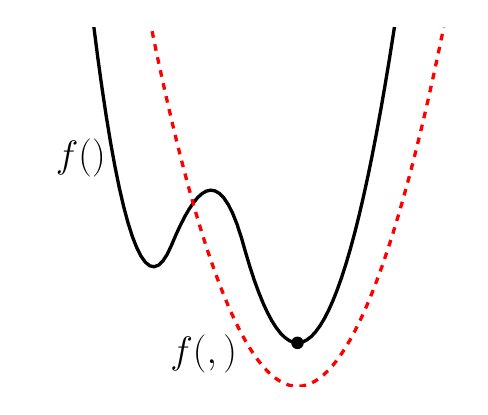
\begin{tikzpicture}[scale=0.8, 
      declare function={
        objective(\x)=      (\x<=-1) * (2*\x*\x + 6*\x + 4)    +
        and(\x>-1, \x<=1) * (\x + 5 - pow(\x,3) - 5*\x*\x) / 4 +
                            (\x>1) * (\x*\x - 5*\x + 4); 
        oracle1(\x)=         (pow(\x - 2.5, 2) / 2 - 3.25);
      }
    ]
    \begin{axis}[
      axis x line=none, axis y line=none,
      ymin=-3.25, ymax=5, ytick={-5,...,5}, ylabel=$y$,
      xmin=-5, xmax=7, xtick={-5,...,7}, xlabel=$x$,
    ]
    \addplot[domain=-5:7, samples=100, objective]{objective(x)};
    \addplot[domain=-5:7, samples=100, oracle]{oracle1(x)};
    
    %% point labels
    \node[label={90:$\wopt$},circle,fill,inner sep=2pt] at (axis cs:2.5,-2.25) {};
    %% function labels
    \node[label={180:$f(\w)$}] at (axis cs:-2.4,2) {};
    \node[label={180:$f(\w, \z)$}] at (axis cs:1.25,-2.5) {};
    \end{axis}
\end{tikzpicture}%
 

            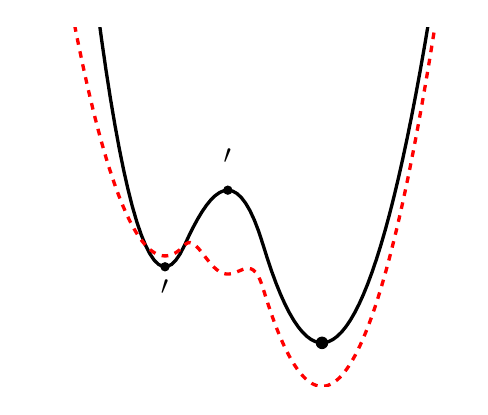
\begin{tikzpicture}[scale=0.8,
      declare function={
        objective(\x)=      (\x<=-1) * (2*\x*\x + 6*\x + 4)    +
        and(\x>-1, \x<=1) * (\x + 5 - pow(\x,3) - 5*\x*\x) / 4 +
                            (\x>1) * (\x*\x - 5*\x + 4); 
        oracle1(\x)=        (\x<=-1) * (pow(x + 1.5, 2))   +
        and(\x>-1, \x<=1) * (-305*pow(\x, 4)/264- 1*pow(\x, 3)/4 + 173*pow(\x,2)/132 - 1*\x/4 - 107/264) +
                            (\x>1) * (pow(x - 2.5, 2) - 3) - 0.25; 
      }
    ]
    \begin{axis}[
      axis x line=none, axis y line=none,
      ymin=-3.25, ymax=5, ytick={-5,...,5}, ylabel=$y$,
      xmin=-5, xmax=6, xtick={-5,...,6}, xlabel=$x$,
    ]
    \addplot[domain=-5:6, samples=100, objective]{objective(x)};
    \addplot[domain=-5:6, samples=200, oracle]{oracle1(x)};
    
    %% point labels
    \node[label={90:$\wopt$},circle,fill,inner sep=2pt] at (axis cs:2.5,-2.25) {};
    \node[label={90:$\w'$},circle,fill,inner sep=1.5pt] at (axis cs:0.1,1.262) {};
    \node[label={270:$\w'$},circle,fill,inner sep=1.5pt] at (axis cs:-1.5,-0.5) {};
    %% function labels
    %\node[label={0:$f(\w)$}] at (axis cs:-2.6,2.5) {};
    %\node[label={180:$f(\w, \z)$}] at (axis cs:1.25,-2.5) {};
    %% plot label
    \end{axis}
\end{tikzpicture}




            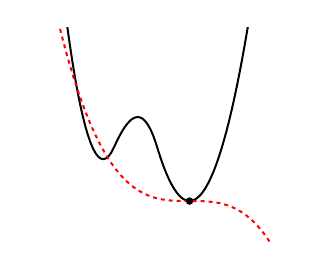
\begin{tikzpicture}[scale=0.48,
      declare function={
        objective(\x)=      (\x<=-1) * (2*\x*\x + 6*\x + 4)    +
        and(\x>-1, \x<=1) * (\x + 5 - pow(\x,3) - 5*\x*\x) / 4 +
                            (\x>1) * (\x*\x - 5*\x + 4); 
        oracle1(\x)=        -(1/30)*pow(x-2.5,3) - 2.25; 
      }
    ]
    \begin{axis}[
      axis x line=none, axis y line=none,
      ymin=-4, ymax=5, ytick={-5,...,5}, ylabel=$y$,
      xmin=-5, xmax=7, xtick={-5,...,7}, xlabel=$x$,
    ]
    \addplot[domain=-5:7, samples=100, objective]{objective(x)};
    \addplot[domain=-5:7, samples=200, oracle]{oracle1(x)};
    
    %% point labels
    \node[label={90:$\wopt$},circle,fill,inner sep=2pt] at (axis cs:2.5,-2.25) {};
    %% function labels
    %\node[label={0:$f(\w)$}] at (axis cs:-2.6,2.5) {};
    %\node[label={180:$f(\w, \z)$}] at (axis cs:1.25,-2.5) {};
    %% plot label
    \end{axis}
\end{tikzpicture}

        \end{minipage}
    \end{frame}

    \begin{frame}{Chapter 2: Interpolation Relationships}

        \begin{itemize}
            \item All three definitions occur in the literature without distinction!
            \item We formally define them and characterize their relationships. 
        \end{itemize}

        \pause

        \begin{restatable}[Interpolation Relationships]{lemma}{interpRelationships}
            Let \( \rbr{f, \oracle{}} \) be arbitrary. 
            Then only the following relationships hold: 
            \begin{align*}
                \text{Minimizer Interpolation} &\implies \text{Mixed Interpolation} \\
                                                                                       & \text{and} &\\
                \text{Stationary-Point Interpolation} &\implies \text{Mixed Interpolation}.
            \end{align*}
            However, if \( f \) and \( f(\cdot, \zk) \) are invex (almost surely) for all \( k \), then the three definitions are equivalent. 
        \end{restatable}

        Note: invexity is weaker than convexity and implied by it. 
        
    \end{frame}
   
    \begin{frame}{Chapter 2: Using Interpolation }
       There are two obvious ways that we can leverage interpolation: 

       \vspace{2ex}

       \begin{enumerate}
           \item Relate interpolation to \textbf{global behavior} of \( \oracle{} \). 
               \vspace{1ex}
               \begin{itemize}
                   \item This was first done using the weak and strong growth conditions by \citet{vaswani2019fast}. 
                \vspace{2ex}
               \end{itemize}
           \item Use interpolation in a \textbf{direct analysis} of SGD. 
               \vspace{1ex}
               \begin{itemize}
                   \item This was first done by \citet{bassily2018exponential}, who analyzed SGD under a curvature condition. 
               \end{itemize}
               \vspace{2ex}
       \end{enumerate}

      We do both, starting with weak/strong growth. 

    \end{frame}

    \begin{frame}{Growth Conditions: Well-behaved Oracles}
        
        \mbox{\large There are many possible regularity assumptions on \oracle{}.} 

        \begin{align*} 
            \textbf{Bounded Gradients}:& \quad  \E\sbr{\norm{\grad(\w, \zk)}^2} \leq \textcolor{red}{\sigma^2}, \\ 
           \intertext{\hspace{3.5em} \small\textbullet{} Proposed by Robbins and Monro in their analysis of SGD. }
           \pause
           \textbf{Bounded Variance}:& \quad \E \sbr{\norm{\grad(\w, \zk)}^2} \leq \textcolor{blue}{\norm{\grad(\w)}^2} + \textcolor{red}{\sigma^2}, \\
           \intertext{\hspace{3.5em} \small \textbullet{} Commonly used in the stochastic approximation setting.}
           \pause
           \textbf{Strong Growth+Noise}:& \quad  \E \sbr{\norm{\grad(\w, \zk)}^2} \leq \rho \, \textcolor{blue}{\norm{\grad(\w)}^2} + \textcolor{red}{\sigma^2}.
           \intertext{\hspace{3.5em} \small \textbullet{} Satisfied when \oracle{} is individually-smooth and bounded below. }
       \end{align*} 

    \end{frame}

    \begin{frame}{Growth Conditions: Strong and Weak Growth}

        \mbox{\large We obtain the strong and weak growth conditions as follows: } 

        \begin{align*} 
            \textbf{Strong Growth+Noise}:& \quad  \E \sbr{\norm{\grad(\w, \zk)}^2} \leq \rho \, \textcolor{blue}{\norm{\grad(\w)}^2} + \textcolor{red}{\sigma^2}. \\
           \intertext{\hspace{3.5em} \small \textbullet{} Does not imply interpolation. }
           \pause
            \textbf{Strong Growth}:& \quad  \E \sbr{\norm{\grad(\w, \zk)}^2} \leq \rho \, \textcolor{blue}{\norm{\grad(\w)}^2}.\\
            \intertext{\hspace{3.5em} \small \textbullet{} Implies \textbf{stationary-point} interpolation. }
           \pause
            \textbf{Weak Growth}:& \quad  \E \sbr{\norm{\grad(\w, \zk)}^2} \leq \alpha \, \textcolor{purple}{\rbr{f(\w) - f(\wopt)}}. 
            \intertext{\hspace{3.5em} \small \textbullet{} Implies \textbf{mixed} interpolation. }
       \end{align*} 

    \begin{textblock}{2.5}(0.3,7)
        \centering
        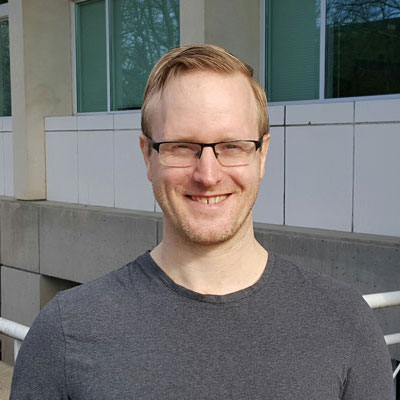
\includegraphics[width=0.4\textwidth]{collaborators/mark}<2->
        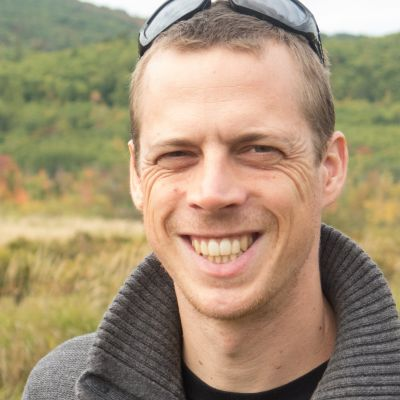
\includegraphics[width=0.4\textwidth]{collaborators/nicolas}<2->
    \end{textblock}

    \begin{textblock}{2.5}(0.3,10)
        \centering
        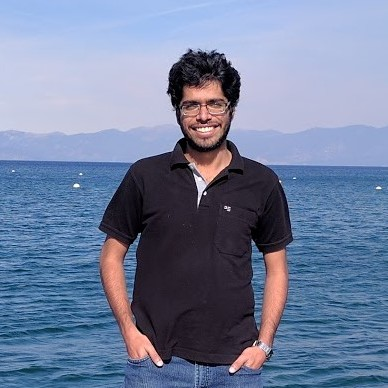
\includegraphics[width=0.4\textwidth]{collaborators/sharan}<3->
        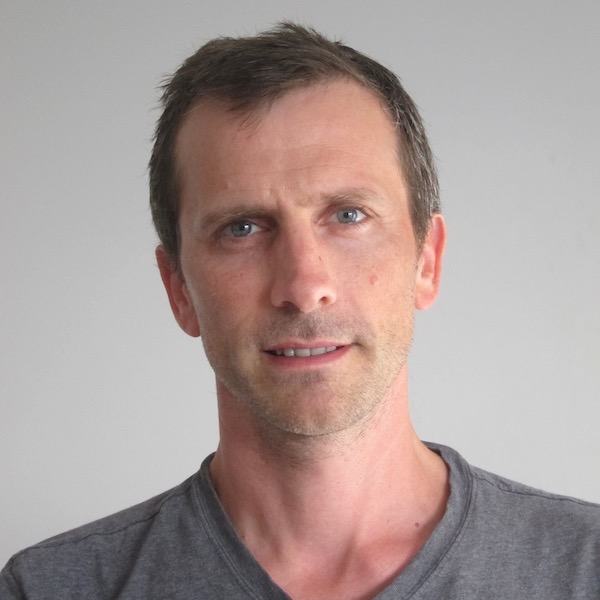
\includegraphics[width=0.4\textwidth]{collaborators/francis}<3->

        \vspace{0.5ex}

        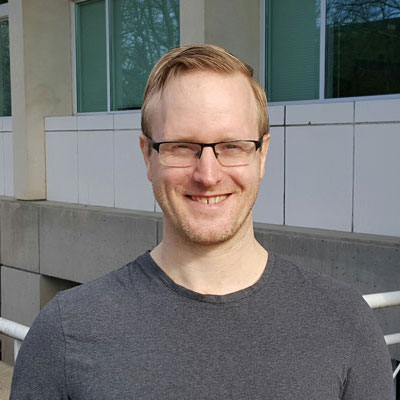
\includegraphics[width=0.4\textwidth]{collaborators/mark}<3->
    \end{textblock}


    \end{frame}

    \begin{frame}{Growth Conditions: Interpolation + Smoothness}
    \begin{center}
            
        \vspace{-2ex}
        \begin{minipage}[t]{0.82\textwidth}
            \vspace{-1.45ex}
            \begin{restatable}[Interpolation and Weak Growth]{lemma}{interpToWGC}~\label{lemma:interpolation-to-wgc}
                Assume \( f \) is \( L \)-smooth and \oracle{} is \( \Lmax \) individually- smooth. 
                If minimizer interpolation holds, then weak growth also holds with
                \( \wgc \leq \frac{L_{\text{max}}}{L}. \)
            \end{restatable}
           

            \begin{restatable}[Interpolation and Strong Growth]{lemma}{interpToSGC}~\label{lemma:interpolation-to-sgc}
                Assume \( f \) is \( L \)-smooth and \( \mu \) strongly-convex and \oracle{} is \( \Lmax \) individually-smooth. 
                If minimizer interpolation holds, then strong growth also holds with 
                \( \rho \leq \frac{L_{\text{max}}}{\mu}. \)
            \end{restatable}
        \end{minipage}
        \begin{minipage}[t]{0.15\textwidth}
            \begin{figure}[t]
                \centering
                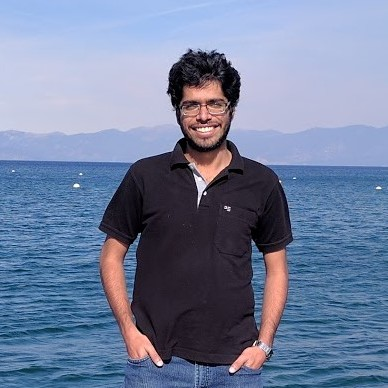
\includegraphics[width=0.8\textwidth]{collaborators/sharan}

                \vspace{0.5ex}

                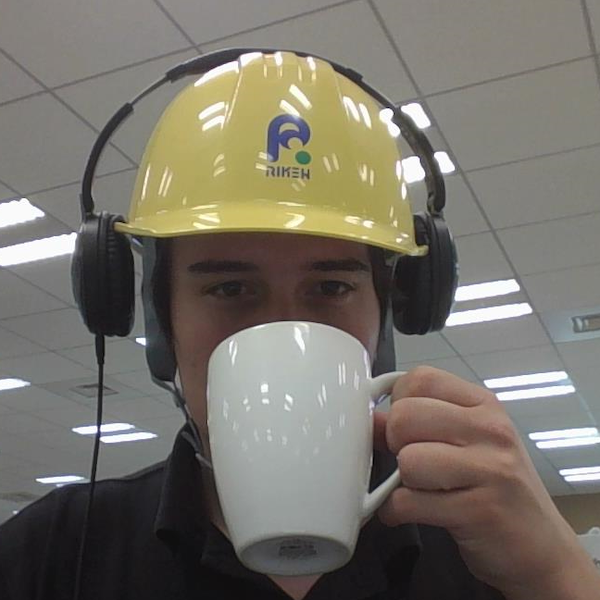
\includegraphics[width=0.8\textwidth]{collaborators/fred}
            \end{figure} 
        \end{minipage}
        
    \end{center}
    \textbf{Comments}:
    \begin{itemize}
        \item This improve on the original result by \citet{vaswani2019fast}, which required convexity.
        \item Oracle framework extends relationship beyond finite-sums. 
        \item See thesis for additional results on weak/strong growth. 
    \end{itemize}

    \end{frame}

    \setbeamercolor{background canvas}{bg=lightcyan}

    \begin{frame}
       \begin{center}
          \huge Chapter 3: Stochastic Gradient Descent\\
       \end{center} 
    \end{frame}
    
    \setbeamercolor{background canvas}{bg=white} 

    \begin{frame}{Chapter 3: Fixed Step-size SGD}
       
        \begin{figure}[t]
        \begin{procedure}{Fixed Step-Size SGD}
        \item Choose an initial point \( \w_0 \in \R^d \).
            \vspace{2ex}
        \item For each iteration \( k \geq 0 \):
            \begin{enumerate}
                \item Query \oracle{} for \( \grad(\wk, \zk) \).
                    \vspace{1ex}
                \item Update input as\vspace{-1ex}%
                    \[ \wkk = \wk - \eta \grad(\wk, \zk). \]
            \end{enumerate}
        \end{procedure}
        \end{figure}


    \end{frame}

    \begin{frame}{Chapter 3: Fixed Step-size SGD}
        
        Prior work for SGD under growth conditions or interpolation: 
        \begin{itemize}
            \item Convergence under strong growth \citep{schmidt2013fast, cevher2018linear}.
            \item Convergence under weak growth \citep{vaswani2019fast}.
            \item Convergence under interpolation \citep{bassily2018exponential}. 
        \end{itemize}
        \vspace{2ex}

       \pause
       \rule{\textwidth}{0.5px}
       \vspace{1ex}

       We still provide many new and improved results! 
       \begin{itemize}
           \item \textbf{Bigger} step-sizes and \textbf{faster} rates for convex and strongly-convex objectives. 
           \item \textbf{Almost-sure} convergence under weak/strong growth. 
           \item \textbf{Trade-offs} between growth conditions and interpolation. 
       \end{itemize}
    \end{frame}


    \setbeamercolor{background canvas}{bg=lightcyan}

    \begin{frame}
       \begin{center}
          \huge Chapter 4: Line Search\\
       \end{center} 
    \end{frame}

    \setbeamercolor{background canvas}{bg=white} 
   
    \begin{frame}{Chapter 4: Weakness of Fixed Step-size SGD}
       \begin{center}
           \Large
           \textbf{Problem}: these convergence rates for fixed step-size SGD rely on using the optimal step-size, which depends on \( \Lmax \), \( \alpha \), or \( \rho \). \\

            \vspace{3ex}
            Is \textbf{grid-search} really the best way to pick \( \eta \)?
       \end{center} 
      
    \begin{figure}[]
        \centering
        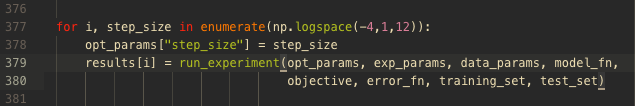
\includegraphics[width=\linewidth]{figures/grid_search}
    \end{figure}

    \end{frame}

    \begin{frame}{SGD:\ the Armijo Line-search}
       
        The \textbf{Armijo line-search} is a classic solution to step-size selection.

        \[ f(\underbrace{\wk - \etak \grad(\wk)}_{\wkk}) \leq f(\wk) - c\cdot \etak \norm{\grad(\wk)}^2. \]
        \vspace{1.2ex}

        \begin{figure}[]
            \centering
            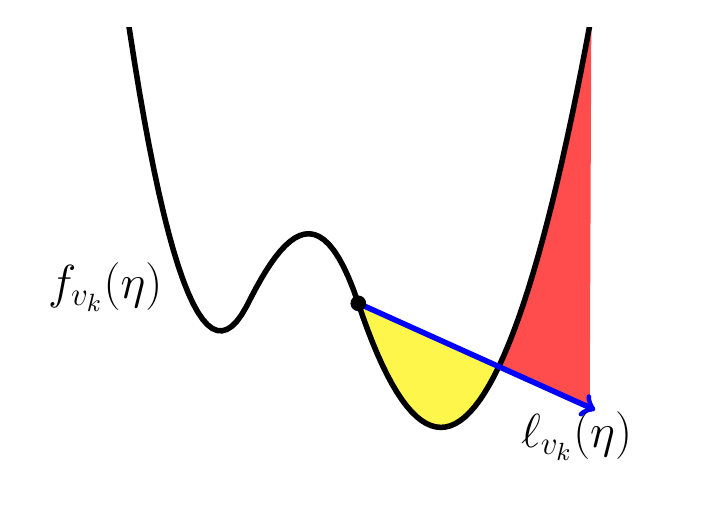
\begin{tikzpicture}[scale=0.9,
      declare function={
        objective(\x)=      (\x<=-1) * (2*\x*\x + 6*\x + 4)    +
        and(\x>-1, \x<=1) * (\x + 5 - pow(\x,3) - 5*\x*\x) / 4 +
                            (\x>1) * (\x*\x - 5*\x + 4); 
        upperBound(\x)=     ( 3*(1 - \x) + 2*pow(\x - 1, 2)); 
        lineSearch(\x)=     ( 0 - 9 * (\x - 1) / 20 ); 
      }
    ]
    \begin{axis}[
      width=0.9\textwidth,
      height=8cm,
      axis x line=none, axis y line=none,
      ymin=-3.25, ymax=5, ytick={-5,...,5}, ylabel=$y$,
      xmin=-5, xmax=7, xtick={-5,...,7}, xlabel=$x$,
    ]

    \addplot[name path=function, domain=-3.5:5.23, samples=100, objective, line width=2pt]{objective(x)};
    \addplot[name path=lineSearch, ->, domain=1:5.3, samples=100, bound, line width=2pt]{lineSearch(x)};
    \addplot[name path=lineSearchEnd, domain=3.55:5.2, samples=20, opacity=0, line width=2pt]{lineSearch(x)};

    \addplot fill between[ 
        of = function and lineSearch, 
        split, % calculate segments
        every even segment/.style = {fill=none},
        every odd segment/.style  = {fill=yellow, fill opacity=0.7}
     ];
    
    \addplot fill between[ 
        of = function and lineSearchEnd, 
        split, % calculate segments
        every even segment/.style = {fill=none},
        every odd segment/.style  = {fill=red, fill opacity=0.7}
     ];

    \node[label={180:$\wk$},circle,fill,inner sep=2pt] at (axis cs:1,0) {};
    
    \node[label={180:$f_{v_k}(\eta)$}] at (axis cs:-2.2,0.3) {};
    \node[label={0:{$\ell_{v_k}(\eta)$}}] at (axis cs:3.6,-2.4) {};
    %\node[label={180:{$h_{v_k}(\eta)$}}] at (axis cs:0.3,3) {};
    \end{axis}
\end{tikzpicture} 

        \end{figure} 
    \end{frame}


    \begin{frame}{SGD with Armijo Line-search: Procedure}
        
        \begin{figure}[t]
            \begin{procedure}{SGD with Armijo Line-Search}
            \item Choose an initial point \( \w_0 \in \R^d \).
                \vspace{1ex}
            \item For each iteration \( k \):
                \begin{enumerate}
                    \item Query \oracle{} for \( f(\wk, \zk), \: \grad(\wk, \zk) \). 
                        \vspace{0.5ex}
                    \item Set \( \etak = \infty \), and \[ \wkk \gets \wk - \etak \grad(\wk, \zk). \]
                    \item Exactly backtrack until
                        \[  \hspace{-1em} f(\wkk, \zk) \leq f(\wk, \zk) - c \cdot \etak \norm{\grad(\wk, \zk)}^2. \]
                \end{enumerate}
            \end{procedure}
        \end{figure}

        Note: Evaluates Armijo condition on \( f(\cdot, \zk) \) instead of \( f \) and needs direct access to \( f(\cdot, \zk) \) to backtrack. 

    \end{frame}

    \begin{frame}{SGD with Armijo Line-search: Visualization}
        \begin{figure}[]
            \centering
            %! TEX root = ../../main.tex
%% Illustration of line-search with and without minimizer interpolation. 

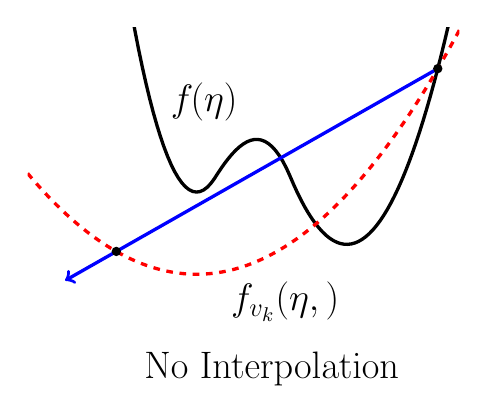
\begin{tikzpicture}[scale=0.8,
      declare function={
        objective(\x)=      (\x<=-1) * (2*\x*\x + 6*\x + 4)    +
        and(\x>-1, \x<=1) * (\x + 5 - pow(\x,3) - 5*\x*\x) / 4 +
                            (\x>1) * (\x*\x - 5*\x + 4); 
        oracle1(\x)=        pow(\x+1.5, 2)/6 - 3.25; 
        lineSearch(\x)=     (\x -4.925) / 1.4 + 3.63;
      }
    ]
    \begin{axis}[
      axis x line=none, axis y line=none,
      ymin=-7, ymax=5, ytick={-5,...,5}, ylabel=$y$,
      xmin=-6, xmax=5.5, xtick={-5,...,7}, xlabel=$x$,
    ]
    \addplot[domain=-4:5.5, samples=100, objective]{objective(x)};
    \addplot[domain=-6:5.5, samples=200, oracle]{oracle1(x)};
    \addplot[<-, domain=-5:4.83, samples=200, bound]{lineSearch(x)};
    
    %% point labels
    %\node[label={90:$\wopt$},circle,fill,inner sep=2pt] at (axis cs:2.5,-2.25) {};
    \node[label={120:$\wk$},circle,fill,inner sep=1.5pt] at (axis cs:4.925,3.63) {};
    \node[label={[label distance=0.3cm] 90:$\wkk$}, circle,fill,inner sep=1.5pt] at (axis cs:-3.639,-2.487) {};
    %% function labels
    \node[label={0:$f_{\vk}(\eta)$}] at (axis cs:-2.6,2.5) {};
    \node[label={340:$f_{v_k}(\eta, \z)$}] at (axis cs:-1,-3.158) {};
    %% plot label
    \node[label={90:No Interpolation}] at (axis cs:0.5,-7.5) {};
    \end{axis}
\end{tikzpicture}%
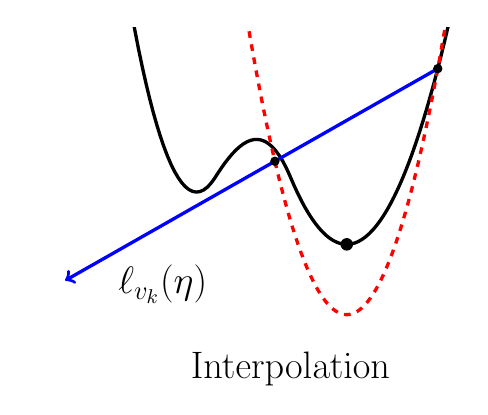
\begin{tikzpicture}[scale=0.8,
      declare function={
        objective(\x)=      (\x<=-1) * (2*\x*\x + 6*\x + 4)    +
        and(\x>-1, \x<=1) * (\x + 5 - pow(\x,3) - 5*\x*\x) / 4 +
                            (\x>1) * (\x*\x - 5*\x + 4); 
        oracle1(\x)=        1.4*pow(\x-2.5, 2) - 4.602; 
        lineSearch(\x)=     (\x -4.925) / 1.4 + 3.63;
      }
    ]
    \begin{axis}[
      axis x line=none, axis y line=none,
      ymin=-7, ymax=5, ytick={-5,...,5}, ylabel=$y$,
      xmin=-6, xmax=5.5, xtick={-5,...,7}, xlabel=$x$,
    ]
    \addplot[domain=-4:5.5, samples=100, objective]{objective(x)};
    \addplot[domain=-6:5.5, samples=200, oracle]{oracle1(x)};
    \addplot[<-, domain=-5:4.83, samples=200, bound]{lineSearch(x)};
    
    %% point labels
    \node[label={270:$\wopt$},circle,fill,inner sep=2pt] at (axis cs:2.5,-2.25) {};
    \node[label={120:$\wk$},circle,fill,inner sep=1.5pt] at (axis cs:4.925,3.63) {};
    \node[label={[label distance=0.3cm] 0:$\wkk$}, circle,fill,inner sep=1.5pt] at (axis cs:0.585,0.53) {};
    %% function labels
    \node[label={355:$\ell_{v_k}(\eta)$}] at (axis cs:-4,-2.645) {};
    %% plot label
    \node[label={90:Interpolation}] at (axis cs:1,-7.5) {};
    \end{axis}
\end{tikzpicture}

        \end{figure} 
    \end{frame}

    \begin{frame}{SGD with Armijo Line-search: Key Lemma}
        \vspace{-2ex}
        \begin{minipage}[t]{0.82\textwidth}
        \vspace{-1.45ex} 
            \begin{restatable}[Step-size Bound]{lemma}{stepSizeBound}~\label{lemma:step-size-bound}
                Assume \( f \) is \( L \)-smooth and \oracle{} is \( \Lmax \) individually- smooth.
                Assume minimizer interpolation holds.\\

                Then the \textbf{maximal} step-size satisfying the stochastic Armijo condition satisfies the following: 
                \[ \frac{2 (1-c)}{\Lmax} \leq \etamax \leq \frac{f(\wk, \zk) - f(\wopt, \zk)}{c \norm{\grad(\wk, \zk)}^2}. \]
            \end{restatable}
            
            \textbf{Comments}:
            \begin{itemize}
                \item Mirrors classic result in deterministic optimization.  
                \item Easy to relax to a backtracking line-search.
            \end{itemize}

       \end{minipage} 
       \begin{minipage}[t]{0.15\textwidth}
            \begin{figure}[t]
                \centering
                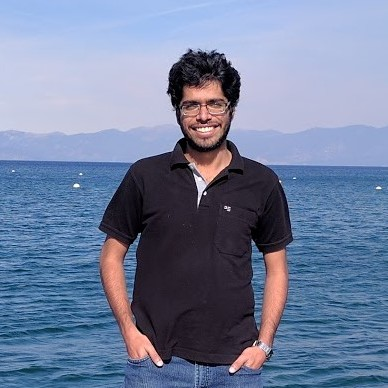
\includegraphics[width=0.8\textwidth]{collaborators/sharan}

                \vspace{0.4ex}
                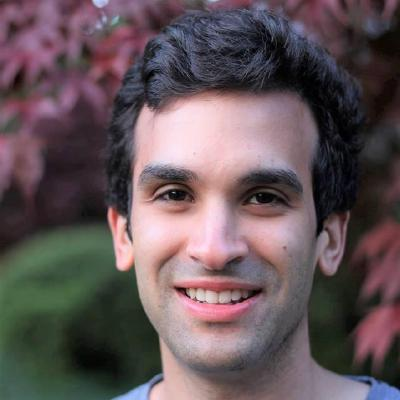
\includegraphics[width=0.8\textwidth]{collaborators/issam}

                \vspace{0.4ex}
                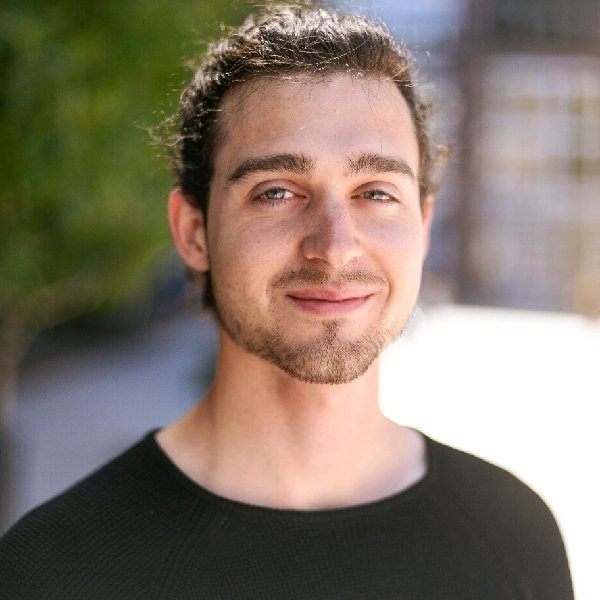
\includegraphics[width=0.8\textwidth]{collaborators/gauthier}

                \vspace{0.4ex}
                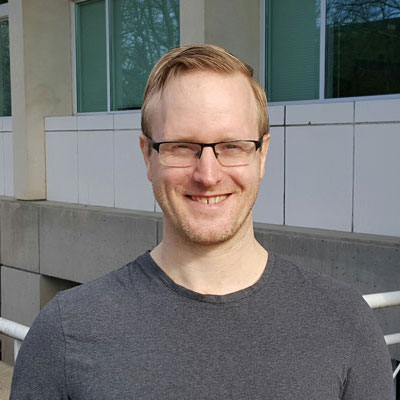
\includegraphics[width=0.8\textwidth]{collaborators/mark}

                \vspace{0.4ex}
                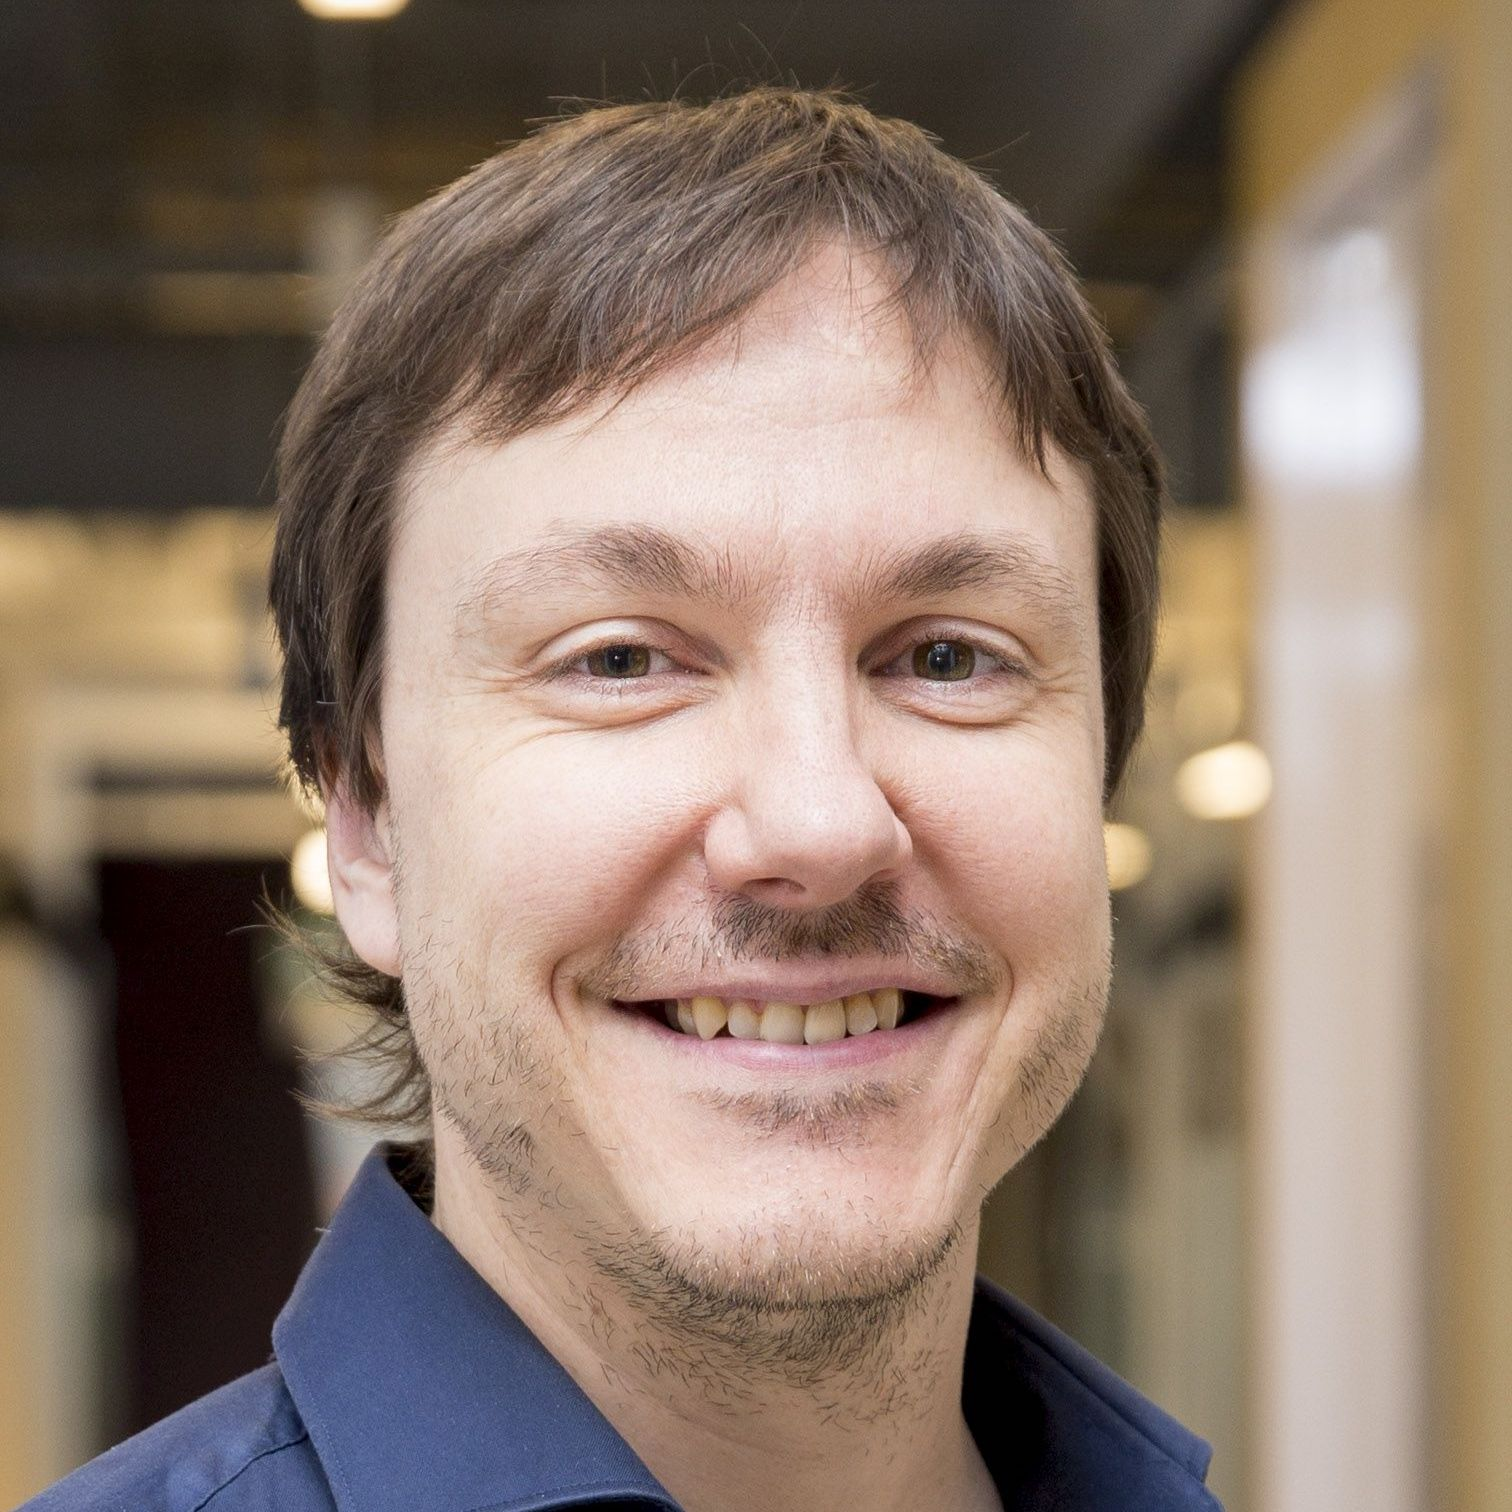
\includegraphics[width=0.8\textwidth]{collaborators/simon}
            \end{figure} 
       \end{minipage}

    \end{frame}

    \begin{frame}{SGD with Armijo Line-Search: Lemma Geometry}
        \Large

        \[  \frac{2 (1-c)}{\Lmax} \leq \etamax \leq \frac{f(\wk, \zk) - f(\wopt, \zk)}{c \norm{\grad(\wk, \zk)}^2}. \] 

        \vspace{1ex} 

        \begin{figure}[]
            \centering
            %! TEX root = ../../main.tex
%% Illustration of step-sizes bound from Armijo line-search. 

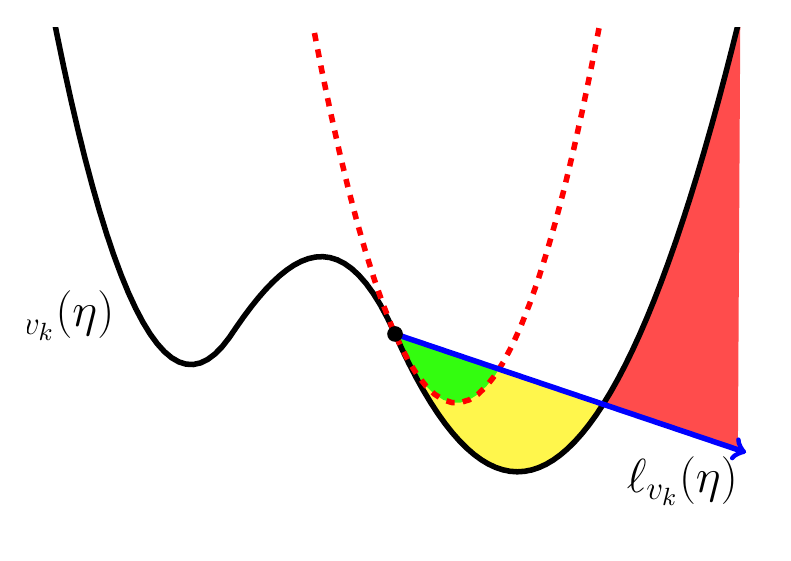
\begin{tikzpicture}[
      declare function={
        objective(\x)=      (\x<=-1) * (2*\x*\x + 6*\x + 4)    +
        and(\x>-1, \x<=1) * (\x + 5 - pow(\x,3) - 5*\x*\x) / 4 +
                            (\x>1) * (\x*\x - 5*\x + 4); 
        upperBound(\x)=     ( 3*(1 - \x) + 2*pow(\x - 1, 2)); 
        lineSearch(\x)=     ( 0 - 9 * (\x - 1) / 20 ); 
      }
    ]
    \begin{axis}[
      width=0.9\textwidth,
      height=8cm,
      axis x line=none, axis y line=none,
      ymin=-3.25, ymax=5, ytick={-5,...,5}, ylabel=$y$,
      xmin=-3.5, xmax=5.5, xtick={-5,...,7}, xlabel=$x$,
    ]

    \addplot[name path=function, domain=-3.5:5.23, samples=100, objective, line width=2pt]{objective(x)};
    \addplot[name path=upperBound, domain=-3.5:7, samples=100, oracle, line width=2pt]{upperBound(x)};
    \addplot[name path=lineSearch, ->, domain=1:5.3, samples=100, bound, line width=2pt]{lineSearch(x)};
    \addplot[name path=lineSearchEnd, domain=3.55:5.2, samples=20, opacity=0, line width=2pt]{lineSearch(x)};

    \addplot fill between[ 
        of = function and lineSearch, 
        split, % calculate segments
        every even segment/.style = {fill=none},
        every odd segment/.style  = {fill=yellow, fill opacity=0.7}
     ];
    
    \addplot fill between[ 
        of = function and lineSearchEnd, 
        split, % calculate segments
        every even segment/.style = {fill=none},
        every odd segment/.style  = {fill=red, fill opacity=0.7}
     ];

    \addplot fill between[ 
        of = upperBound and lineSearch, 
        split, % calculate segments
        every even segment/.style = {fill=none},
        every odd segment/.style  = {fill=green, fill opacity=0.8}
     ];
    \node[label={180:$\wk$},circle,fill,inner sep=2pt] at (axis cs:1,0) {};
    
    \node[label={180:$f_{v_k}(\eta)$}] at (axis cs:-2.2,0.3) {};
    \node[label={0:{$\ell_{v_k}(\eta)$}}] at (axis cs:3.6,-2.4) {};
    %\node[label={180:{$h_{v_k}(\eta)$}}] at (axis cs:0.3,3) {};
    \end{axis}
\end{tikzpicture} 

        \end{figure} 

    \end{frame}

    \begin{frame}{SGD with Armijo Line-search: Convergence}
        \begin{restatable}[Convex + Interpolation]{theorem}{convexLineSearch}~\label{thm:convex-line-search}
            Assume \( f \) is convex, \( L \)-smooth and \( \oracle{} \) is \( \Lmax \) individually-smooth.
            Assume minimizer interpolation holds and \( \f(\cdot, \zk) \) is almost-surely convex for all \( k \).
            Then SGD with the Armijo line-search and \( c = \half \) converges as 
            \begin{align*}
                \E\sbr{f(\bar \w_K)} - f(\wopt) &\leq \frac{\Lmax}{2 \, K} \norm{\w_0 - \wopt}^2.
            \end{align*} 
        \end{restatable}
        
        \textbf{Comments}:
        \begin{itemize}
            \item Improves constants in original result \citep{vaswani2019painless} ---
            line-search is just as fast as the best constant step-size! 
            \item Using the Armijo line-search is (nearly) parameter-free and recovers the deterministic rate when \( \Lmax = L \). 
            \item See thesis for strongly-convex rate (improves \( \bar \mu \) to \( \mu \)). 
        \end{itemize}

    \end{frame}


    \setbeamercolor{background canvas}{bg=lightcyan}

    \begin{frame}
       \begin{center}
          \huge Chapter 5: Acceleration \\
       \end{center} 
    \end{frame}
    

    \setbeamercolor{background canvas}{bg=white}


    \begin{frame}{Chapters 5 and 6: Acceleration}

       SGD can be accelerated when minimizer interpolation holds:
       \begin{itemize}
           \item \citet{liu2020accelerating} modify Nesterov's method and analyze convergence for strongly-convex functions. 
      \vspace{1ex}
           \item \citet{vaswani2019fast} analyze Nesterov's method under strong growth for strongly-convex and convex functions. 
       \end{itemize}

      \vspace{2ex}
      We follow \citet{vaswani2019fast}, but provide tighter rates. 
      \begin{itemize}
          \item Improves dependence on the strong-growth parameter from \( \rho \) to \( \sqrt{\rho} \) --- factor of \( \sqrt{\Lmax / \mu} \) in the worst case. 
        \vspace{1ex}
          \item Analysis proceeds via estimating sequences; details in thesis.  
      \end{itemize}
        
    \end{frame}

    \begin{frame}{Recap}
       \begin{center}
         \vspace{-2ex}
         \Large Takeaways.

         \vspace{-1ex}
         \rule{0.66\textwidth}{1px}
         \vspace{1ex}
       \end{center}

        \begin{itemize}
            \item \textbf{Interpolation}: the oracle model is extends interpolation to general stochastic optimization problems. 
                \vspace{1ex}
            \item \textbf{Growth Conditions}: ``smooth'' oracles satisfying interpolation are well-behaved globally. 
                \vspace{1ex}
            \item \textbf{SGD}: improved rates show SGD under interpolation is tight with the deterministic case. 
                \vspace{1ex}
            \item \textbf{Line-Search}: the Armijo line-search yields fast, parameter-free optimization under interpolation.  
                \vspace{1ex}
            \item \textbf{Acceleration}: stochastic acceleration is possible with a penalty of only \( \sqrt{\rho} \). 
        \end{itemize}
    \end{frame}
    
    \setbeamercolor{background canvas}{bg=white}

    %% end slide
    \setbeamercolor{background canvas}{bg=lightcyan}

    \begin{frame}{}
        \begin{center}
        \huge Thanks for Listening!
        \end{center}
    \end{frame}

    \setbeamercolor{background canvas}{bg=white}


    \begin{frame}{Acknowledgements}
     
        \begin{figure}
            \centering
            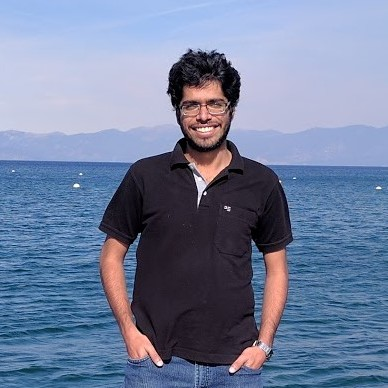
\includegraphics[width=0.18\textwidth]{collaborators/sharan}
            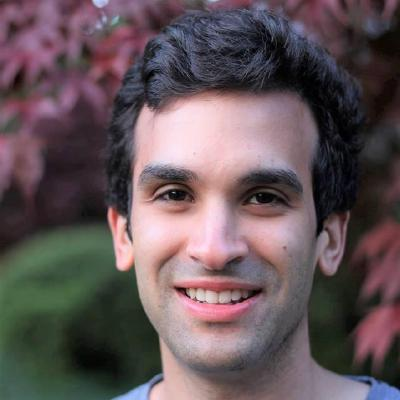
\includegraphics[width=0.18\textwidth]{collaborators/issam}
            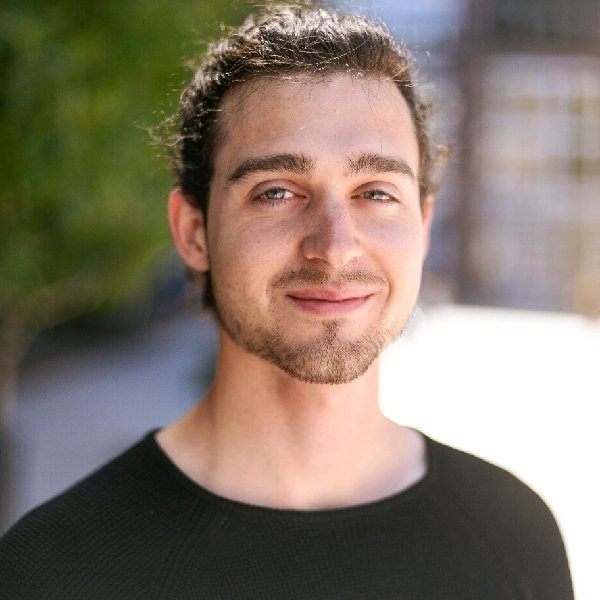
\includegraphics[width=0.18\textwidth]{collaborators/gauthier}
            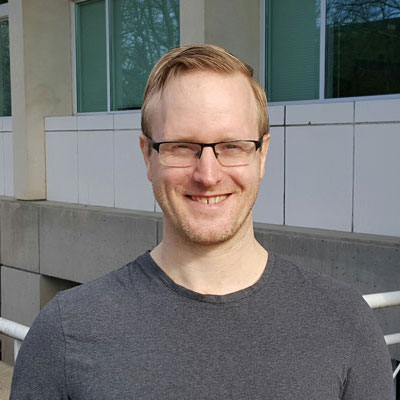
\includegraphics[width=0.18\textwidth]{collaborators/mark}
            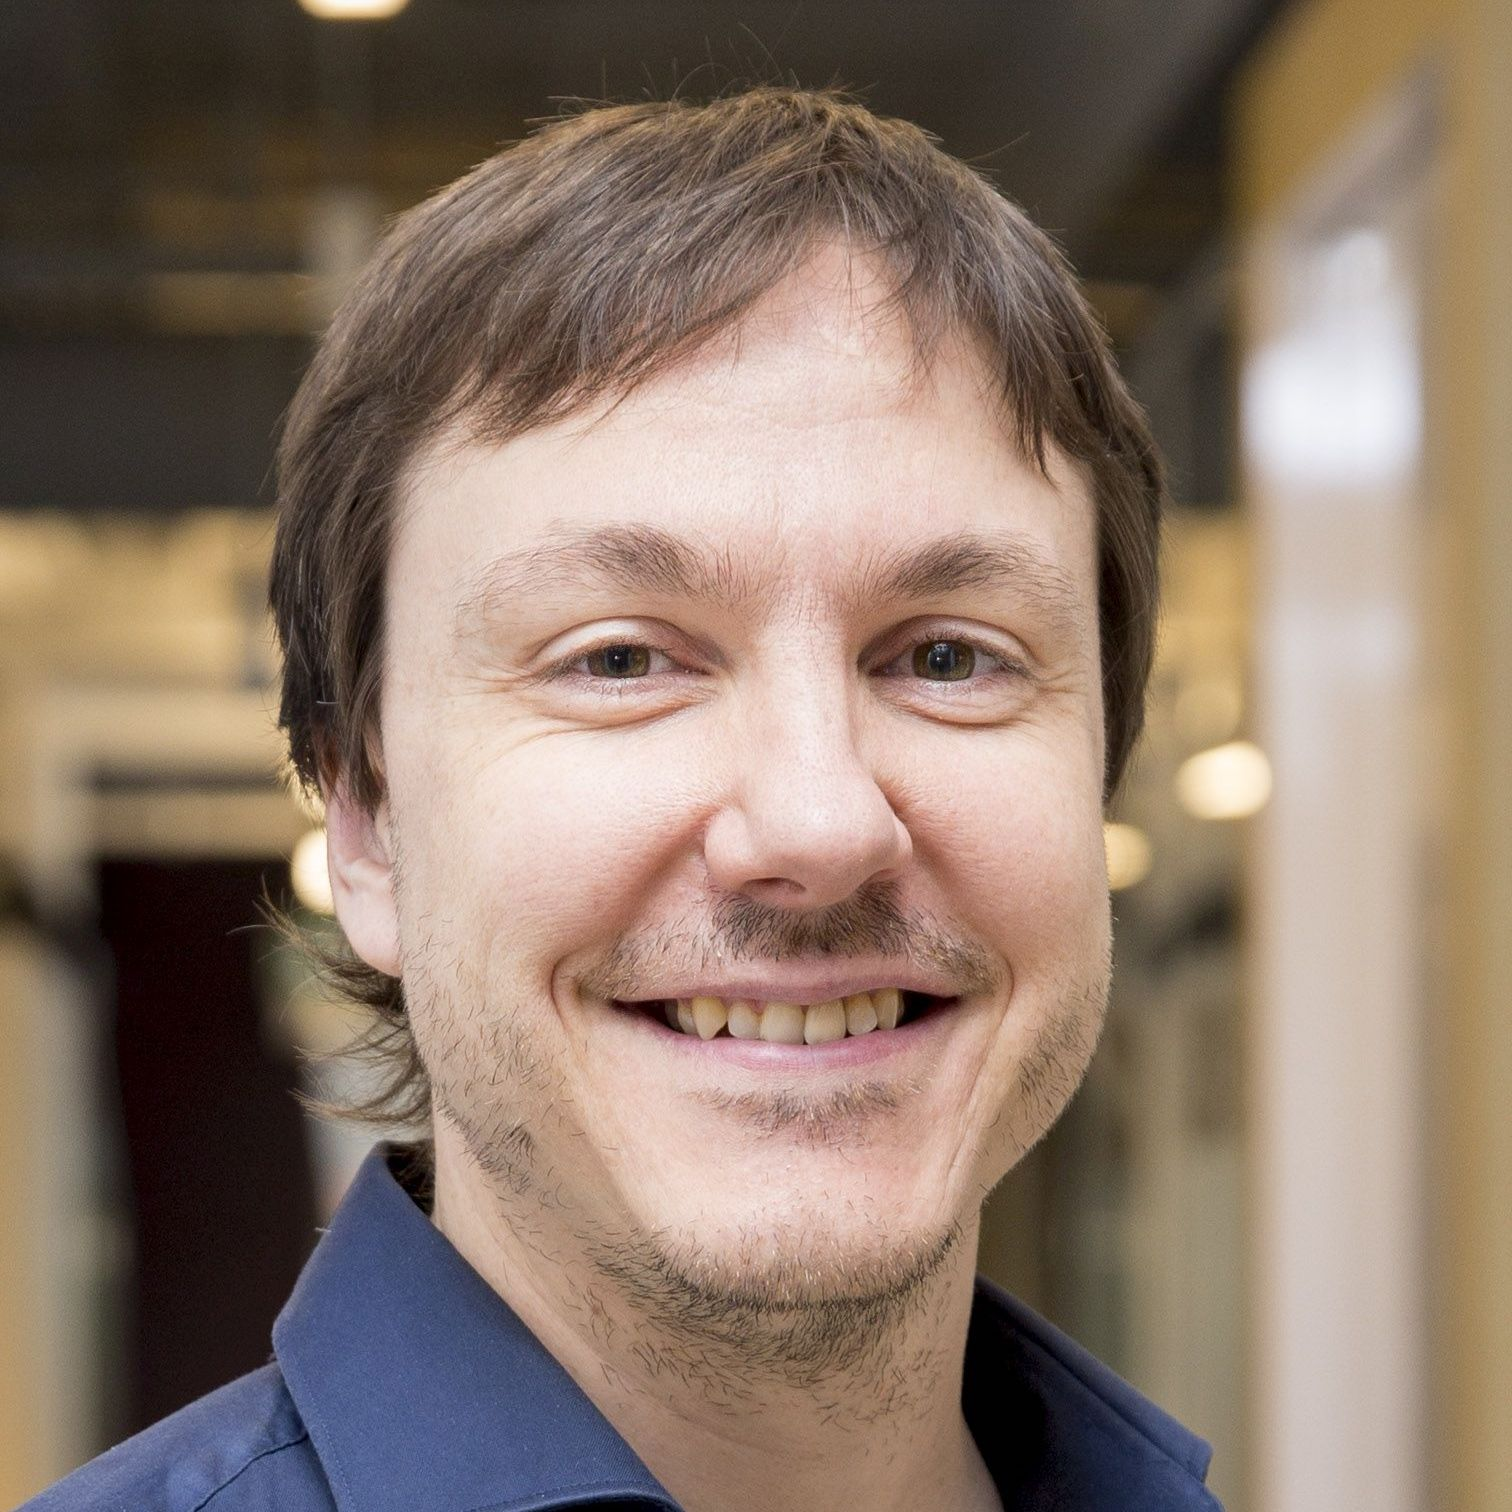
\includegraphics[width=0.18\textwidth]{collaborators/simon}

            \vspace{0.4ex}%

            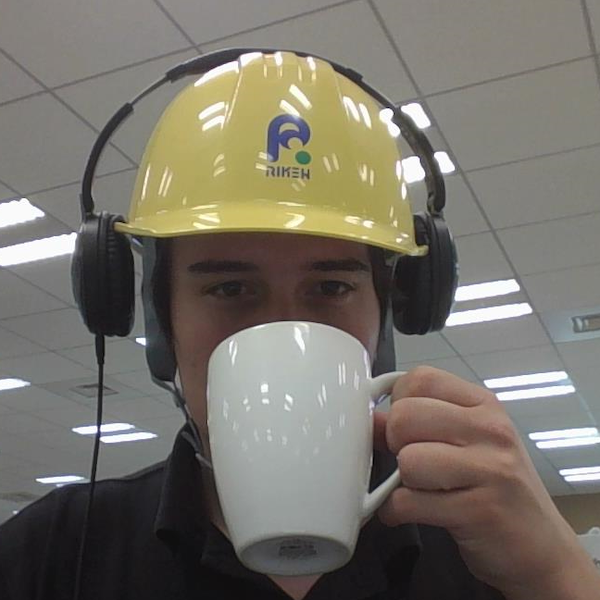
\includegraphics[width=0.18\textwidth]{collaborators/fred}
            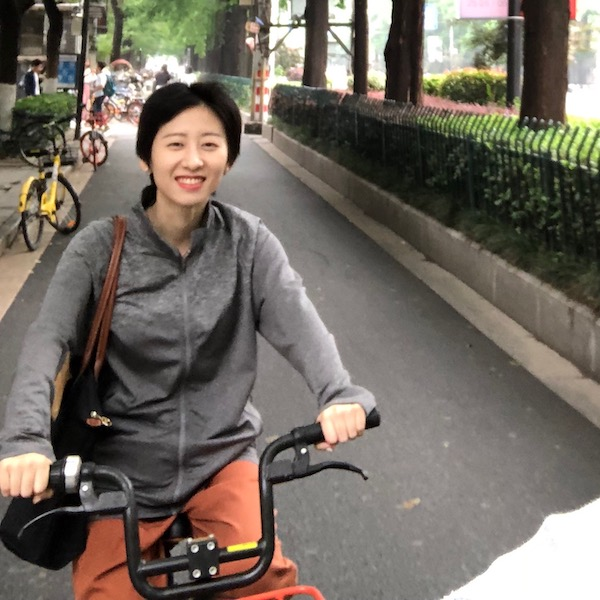
\includegraphics[width=0.18\textwidth]{collaborators/cathy}
            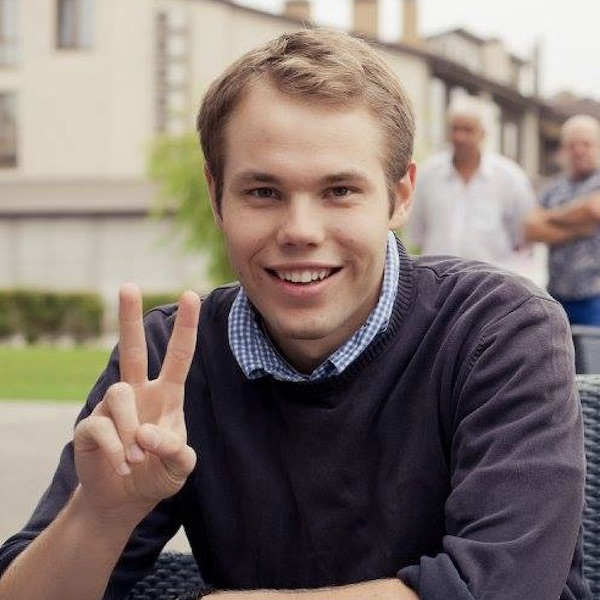
\includegraphics[width=0.18\textwidth]{collaborators/wilder}
            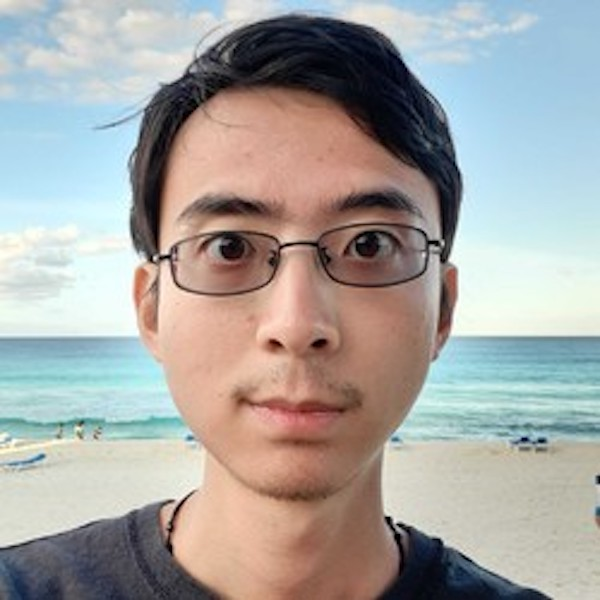
\includegraphics[width=0.18\textwidth]{collaborators/joey}
        \end{figure}

        \textbf{Left to right}:
            \href{https://vaswanis.github.io/}{Sharan Vaswani}, \href{https://issamlaradji.github.io/}{Issam Laradji}, \href{https://gauthiergidel.github.io/}{Gauthier Gidel}, \href{https://www.cs.ubc.ca/~schmidtm/}{Mark Schmidt}, \href{http://www.iro.umontreal.ca/~slacoste/}{Simon Lacoste-Julien}, \href{https://fkunstner.github.io/}{Frederik Kunstner}, \href{https://www.cs.ubc.ca/~mengxixi/}{Si Yi Meng}, \href{https://wilderlavington.github.io/}{Jonathan Lavington}, \href{https://joeyandbluewhale.github.io/}{Yihan Zhou}, and Betty Shea. 
    
        \end{frame}

        \begin{frame}{Bonus: SFOs and Least Squares}
        \vspace{-1ex}

        \[ \textbf{Least Squares}: \wopt \in \argmin \frac{1}{2n} \sum_{i=1}^n \rbr{\abr{w, x_i} - y_i}^2. \]
        
        \vspace{2ex} 
        
        The \textbf{sub-sampling} oracle sets \( \zk \sim \text{Uniform}(1, \ldots, n) \) and returns 
        \[ f(\w, \zk) =  \half \rbr{\abr{w, x_i} - y_i}^2 \quad \text{and} \quad \grad(\wk, \zk) = \rbr{\abr{\w, x_i} - y_i} x_i. \]

        \pause 
        \rule{\textwidth}{0.4pt}
        Observations: 
        \begin{itemize}
            \item \textcolor{red}{\oracle{} is \textbf{unbiased}.} 
            \item \textcolor{blue}{\oracle{} is \( \Lmax = \max_{i} \norm{x_i}^2_2 \) \textbf{individually-smooth}} since 
                    \[ f_{i}(\w) = \half \rbr{\abr{w, x_{i}} - y_{i}}^2, \]
                    is \( \norm{x_{i}}_2^2 \)-smooth for each \( i \in [n] \).
        \end{itemize}

    \end{frame}


    \begin{frame}{Bonus: Convergence for Fixed Step-size SGD}
        \begin{restatable}[Convex + Weak Growth]{theorem}{wgcConvex}~\label{thm:wgc-convex}
            Assume \( f \) is convex, \( L \)-smooth and \( \rbr{f, \oracle{}} \) satisfies weak growth. 
            Then SGD with \( \eta = \frac{1}{2 \wgc L} \) converges as
            \[ \E\sbr{\f(\bar \w_K)} - f(\wopt) \leq \frac{2 \alpha L}{K} \norm{\w_0 - \wopt}^2. \]
        \end{restatable}

        \begin{restatable}[Convex + Interpolation]{theorem}{wgcConvexIndSmooth}~\label{thm:wgc-convex-ind-smooth}
            Assume \( f \) is convex, \( L \)-smooth and \oracle{} is \( \Lmax \) individually-smooth. 
            Assume minimizer interpolation holds. 
            Then SGD with \( \eta = \frac{1}{\Lmax} \) converges as
            \[ \E\sbr{f(\bar w_K)} - f(\wopt) \leq \frac{\Lmax}{2 \, K} \norm{\w_0 - \wopt}^2.   \]
        \end{restatable}
    \end{frame}

    \begin{frame}{Bonus: Trade-offs}
       \vspace{-2ex}
       \begin{align*}
           \textbf{Weak Growth}:  \quad \E\sbr{\f(\bar \w_K)} - f(\wopt) &\leq \frac{2 \alpha L}{K} \norm{\w_0 - \wopt}^2.
            \intertext{\hspace{13em} \Large v.s.}
            \textbf{Interpolation}: \quad \E\sbr{f(\bar \w_K)} - f(\wopt) &\leq \frac{\Lmax}{2 \, K} \norm{\w_0 - \wopt}^2.\\
       \end{align*} 

        \textbf{Comments:}
        \begin{itemize}
            \item By minimizer interpolation and individual-smoothness, 
                \[ \alpha \leq \frac{\Lmax}{L}. \]
            \item So, the second rate is better than the first in the \textbf{worst-case}!  
            \item If \( \Lmax = L \), then the second rate is tight deterministic GD!
        \end{itemize}
    \end{frame}

    %% bibliography
    \begin{frame}[allowframebreaks]{References}
        \bibliographystyle{plainnat}
        \bibliography{refs}
    \end{frame}


\end{document}
